\documentclass[12pt,oneside,openany]{report}

% Page geometry
\usepackage[a4paper,left=2.0cm,right=2.25cm,top=2.25cm,bottom=2.25cm]{geometry}

% Fonts and symbols
\usepackage{fontawesome5}
\usepackage{fontspec}
\setmainfont{Arial} % or replace with Garamond/libertine/Garamond, etc.
\usepackage{amssymb}
\usepackage{emoji}

% Lists and enumerations
\usepackage{enumitem}

% Math and graphics
\usepackage{graphicx}
\usepackage{tikz}
\usetikzlibrary{3d, shapes.geometric, arrows.meta, positioning}
\usepackage{pgfplots}
\pgfplotsset{compat=1.18}

\usepackage[absolute]{textpos}

% Colors and backgrounds
\usepackage{xcolor}
\usepackage{pagecolor}
\definecolor{tutorialbg}{RGB}{245,245,240}
\definecolor{assignmentbg}{RGB}{240,248,255}
\definecolor{stardustbg}{RGB}{225,246,255}
\definecolor{pastelyellowbg}{RGB}{255,255,245}
\definecolor{nav}{rgb}{0.00, 0.2, 0.4}
\definecolor{mrn}{rgb}{0.52, 0.0, 0.0}
\definecolor{blu}{rgb}{0.52, 0.1, 1.0}

% Hyperlinks
\usepackage{hyperref}
\hypersetup{
    colorlinks,
    citecolor=nav,
    filecolor=mrn,
    linkcolor=mrn,
    urlcolor=mrn
}

% Custom box
\usepackage[most]{tcolorbox}
\newtcolorbox{mytextbox}[1][]{%
  sharp corners,
  enhanced,
  colback=white,
  height=10cm,
  attach title to upper,
  #1
}

% Algorithms and code
\usepackage{algorithm}
\usepackage{algpseudocode}
\usepackage{listings}
\definecolor{codegray}{gray}{0.9}
\definecolor{codered}{rgb}{0.6,0,0}
\definecolor{codeblue}{rgb}{0,0,0.6}
\lstdefinestyle{mystyle}{
  backgroundcolor=\color{codegray},
  commentstyle=\color{codered},
  keywordstyle=\color{codeblue},
  numberstyle=\tiny\color{gray},
  stringstyle=\color{purple},
  basicstyle=\ttfamily\footnotesize,
  breakatwhitespace=false,
  breaklines=true,
  captionpos=b,
  keepspaces=true,
  numbers=left,
  numbersep=5pt,
  showspaces=false,
  showstringspaces=false,
  showtabs=false,
  tabsize=2
}
\lstset{style=mystyle, language=Python}

% Styling chapters and sections
\usepackage{sectsty}
\chapterfont{\color{mrn}}
\partfont{\color{mrn}}
\sectionfont{\color{nav}}
\subsectionfont{\color{nav}}
\subsubsectionfont{\color{nav}}

% Title and TOC formatting
\renewcommand{\contentsname}{\hfill </.{\it Table of Contents} >}
\setcounter{tocdepth}{1}

% Fancy header/footer
\usepackage{fancyhdr}
\pagestyle{fancy}
\fancyhf{}
\fancyhead[R]{\color{mrn}\thesection}
\fancyfoot[R]{\color{gray} {\it \small Lecture Notes by Hemant, K.} \hspace{0.1em}\color{mrn} | \thepage}
\renewcommand{\headrulewidth}{0pt}
\renewcommand{\footrulewidth}{0pt}
\fancypagestyle{plain}{%
  \fancyhf{}
  \fancyfoot[R]{\color{lightgray}\thepage}
  \renewcommand{\headrulewidth}{0pt}
  \renewcommand{\footrulewidth}{0pt}
}

% Part/chapter/section formatting
\usepackage{chngcntr}
\counterwithin*{chapter}{part}
\renewcommand{\thepart}{\arabic{part}}
\renewcommand\thechapter{\arabic{chapter}} %\thepart.\arabic{chapter}}
\renewcommand\thesection{\thechapter.\arabic{section}} %\thechapter.\arabic{section}}
\renewcommand\thesubsection{\thesection.\arabic{subsection}} %\thesection.\arabic{subsection}}
\renewcommand\partname{Week}
\renewcommand{\chaptername}{>> Lecture /}

% Appendix formatting
\let\oldappendix\appendix
\renewcommand{\appendix}{
    \renewcommand{\thesection}{\alph{section}}
    \oldappendix}

% Tables
\usepackage{tabularx}
\usepackage{array}
\usepackage{booktabs}
\usepackage{bookmark}

% Font
\usepackage{libertine} % Libertine font family

% Line spacing
\usepackage{parskip}

% Title setup
%%%-----------------------------------------------------------------------------------%%%
\title{\color{mrn} \Huge \bfseries  $\faWifi$ Beyond 5G: Foundations and Future of Mobile Communication $\faWifi$  \\ {\it Lecture Notes and Exercises on 5G and 6G Technologies}}
\author{Hemant, K.} 
\date{
\makebox[\textwidth]{
\includegraphics[width=1.0\paperwidth]{./figures/5g6g.png}}
}
% Document begins
%%%-----------------------------------------------------------------------------------%%%
\begin{document}  
\sloppy  % This will apply sloppy line-breaking to the entire document
\pagecolor{stardustbg}
\maketitle
\clearpage
% \pagecolor{white}
%%%-----------------------------------------------------------------------------------%%%

\thispagestyle{empty}
% Copyright Page

{\small
\setlength{\parindent}{0em}\setlength{\parskip}{1em}

~

\vfill

\begin{center}
  
\includegraphics[width=0.25\textwidth]{figures/open-book-icon.png}\\[1em]
  
\includegraphics[width=0.35\textwidth]{figures/cc-by-nc-nd.png}
\end{center}

\vspace{1em}

Copyright \copyright{} 2025 Kumar Hemant

All rights reserved. No part of this journal may be reproduced, stored, or transmitted in any form or by any means—electronic, mechanical, photocopying, recording, scanning, or otherwise—without written permission from the author. It is illegal to copy this journal, post it to a website, or distribute it by any other means without permission.

This journal is a personal learning resource and is intended for academic and educational purposes only. Any resemblance to course content or proprietary material is coincidental and unintentional.

Licensed under a [Creative Commons Attribution-NonCommercial-NoDerivatives 4.0 International License](https://creativecommons.org/licenses/by-nc-nd/4.0/).

First edition, 2025

Published by Kumar Hemant


% % Copyright Page

% {\small
% \setlength{\parindent}{0em}\setlength{\parskip}{1em}

% ~

% \vfill

% Copyright \copyright{} 2025 Kumar Hemant

% All rights reserved. No part of this journal may be reproduced, stored, or transmitted in any form or by any means—electronic, mechanical, photocopying, recording, scanning, or otherwise—without written permission from the author. It is illegal to copy this journal, post it to a website, or distribute it by any other means without permission.

% This journal is a personal learning resource and is intended for academic and educational purposes only. Any resemblance to course content or proprietary material is coincidental and unintentional.

% First edition, 2025

% Published by Kumar Hemant  

\clearpage
\pagecolor{white}

\tableofcontents

% #📘 chapter1.tex — Introduction to Wireless Communication

% 🗂 Assets You’ll Need:
% Asset   Description
% notebooks/A1-signal_strength.ipynb  Notebook simulating signal strength over distance
% figures/fspl_plot.png   Save a path loss graph image
% Streamlit App Page 1    We'll create this next for CellCoverage.py


\chapter{Introduction to Wireless Communication}

\section{Cellular Network Fundamentals}

\subsection{What is Wireless Communication?}
Wireless communication refers to the transfer of information between two or more points that are not physically connected. It forms the basis for mobile networks, enabling services like voice calling, mobile data, and SMS.

\subsection{Basic Terminology}
\begin{itemize}
    \item \textbf{Base Station (BS)}: The fixed point of communication for mobile devices in a cell.
    \item \textbf{User Equipment (UE)}: Devices such as smartphones and modems.
    \item \textbf{Radio Access Network (RAN)}: Connects UE to the core network.
    \item \textbf{Frequency Band}: The range of frequencies used for wireless transmission.
\end{itemize}

\section{Generations of Mobile Networks}

\subsection{From 1G to 5G}
\begin{itemize}
    \item \textbf{1G}: Analog voice only, poor quality and security.
    \item \textbf{2G}: Digital voice (GSM), SMS, and limited data (GPRS, EDGE).
    \item \textbf{3G}: Mobile broadband (UMTS, HSPA), video calling.
    \item \textbf{4G}: All-IP network (LTE), high-speed data, VoLTE.
    \item \textbf{5G}: Massive MIMO, mmWave, URLLC, eMBB, mMTC.
\end{itemize}

\subsection{Key Performance Metrics}
\begin{itemize}
    \item \textbf{Latency}: Time delay in communication.
    \item \textbf{Throughput}: Amount of data transferred per second.
    \item \textbf{Spectral Efficiency}: Bits/sec/Hz — how efficiently spectrum is used.
    \item \textbf{Energy Efficiency}: Data transmitted per joule of energy.
\end{itemize}

\section{The Cellular Concept}

\subsection{Cell Reuse and Frequency Planning}
Cellular systems divide the service area into small regions (cells) each with a base station, and reuse frequency bands in a planned manner to avoid interference.

\subsection{Hexagonal Cell Approximation}
\begin{itemize}
    \item Provides a geometrical model for coverage.
    \item Each cell uses a different set of frequencies compared to its neighbors.
    \item Reuse Factor $N = i^2 + ij + j^2$ where $(i,j)$ are frequency reuse parameters.
\end{itemize}

\subsection{Interference and SINR}
The performance of wireless communication depends on the Signal to Interference plus Noise Ratio (SINR). Techniques such as sectorization, power control, and handover are used to manage interference.

\section{Visualizing Wireless Signals}

\subsection{Path Loss Models}
\begin{itemize}
    \item \textbf{Free Space Path Loss (FSPL)}: 
    \[
    \text{FSPL (dB)} = 20 \log_{10}(d) + 20 \log_{10}(f) + 20 \log_{10}\left(\frac{4\pi}{c}\right)
    \]
    \item \textbf{Log-distance path loss}: 
    \[
    PL(d) = PL(d_0) + 10n \log_{10}\left(\frac{d}{d_0}\right)
    \]
\end{itemize}

\subsection{Interactive Visualizations (Notebook/Streamlit)}
See Appendix~\ref{appendix:A1} and Appendix~\ref{appendix:A2} for interactive notebooks and streamlit apps.

\section{Summary}
This chapter introduced basic concepts in wireless communication including the evolution of mobile generations, the cellular concept, and essential performance metrics.

\section{Further Reading}
\begin{itemize}
    \item T. S. Rappaport, \textit{Wireless Communications: Principles and Practice}, Prentice Hall.
    \item Andreas F. Molisch, \textit{Wireless Communications}, Wiley.
    \item 3GPP TS 38.300: 5G NR Overall Architecture.
\end{itemize}

% \appendix

% \chapter*{Appendices}
% \addcontentsline{toc}{chapter}{Appendices}

\section{Appendix A1: Signal Strength and Path Loss Notebook}
\label{appendix:A1}
\textbf{Download:} \texttt{notebooks/A1-signal\_strength.ipynb} \\
\textbf{Topics Covered:} Free space path loss, signal visualization in dBm vs distance. \\
\textbf{Preview:}  
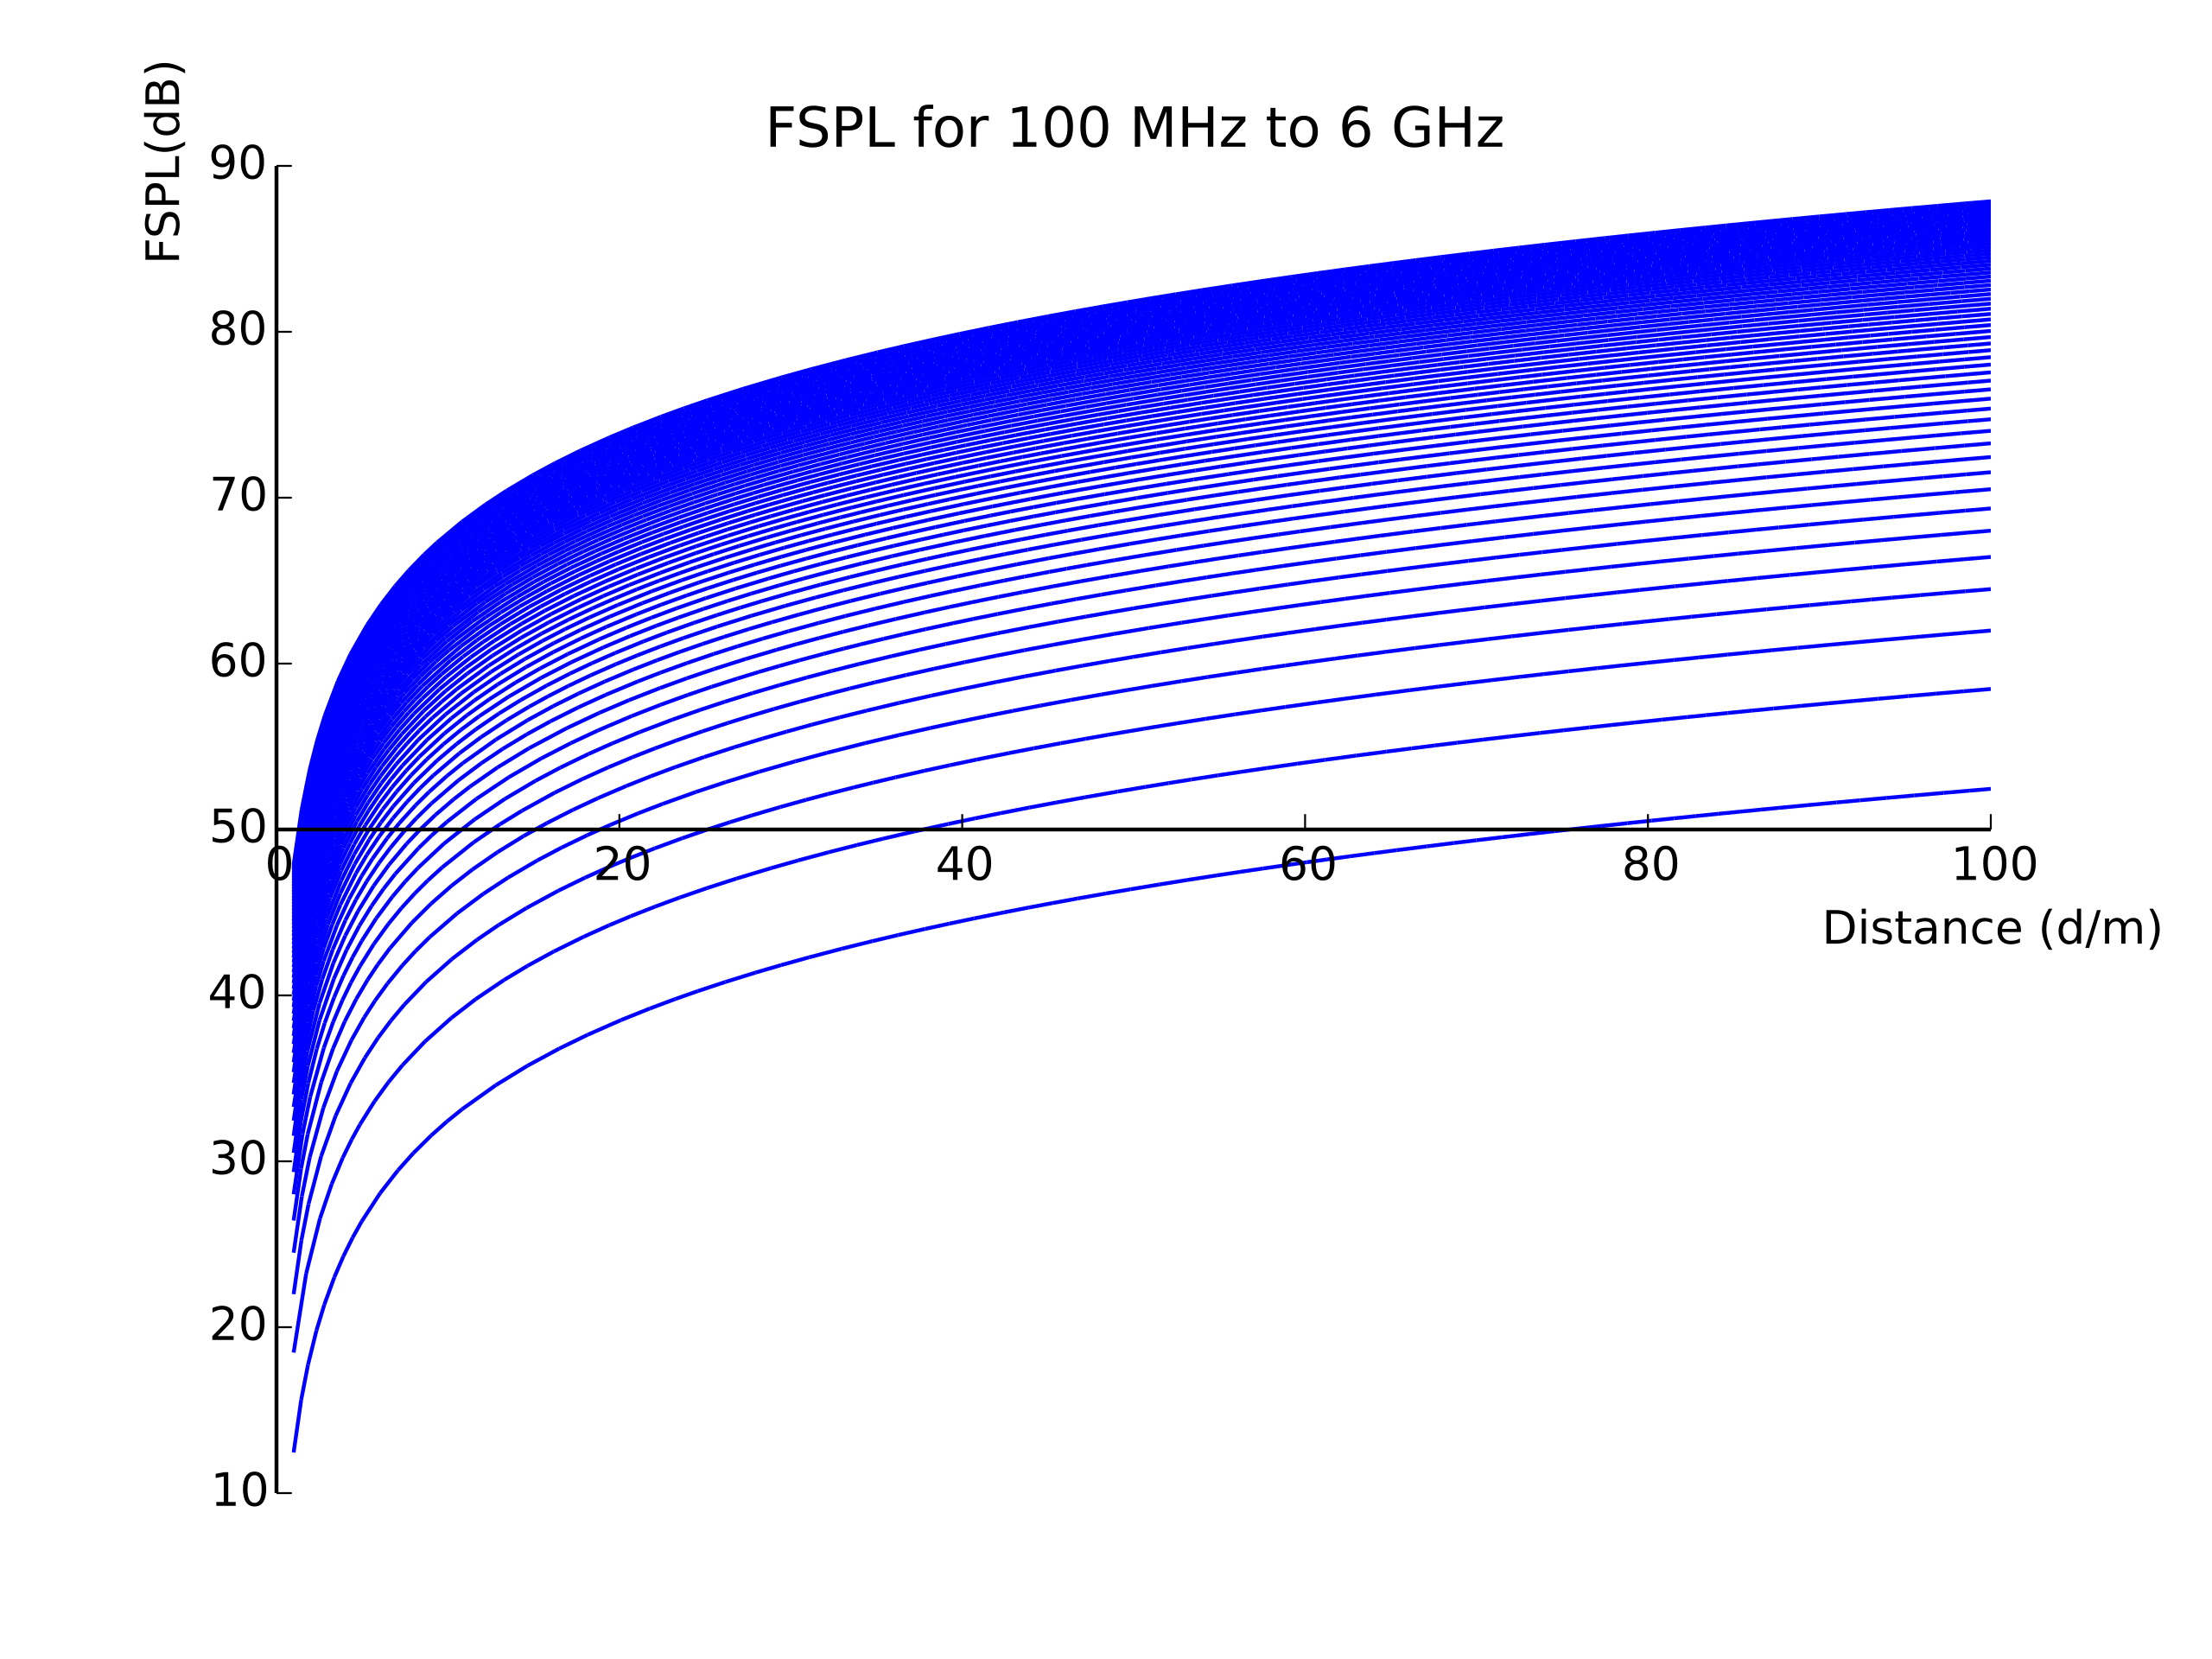
\includegraphics[width=0.9\textwidth]{./images/fspl_plot.png}

\section{Appendix A2: Streamlit App – Cell Coverage Planner}
\label{appendix:A2}
\textbf{URL:} \url{http://localhost:8501/CellCoverage} \\
\textbf{Features:} 
\begin{itemize}
    \item Adjust cell radius and visualize overlapping coverage.
    \item Frequency reuse simulation with color-coded hex cells.
    \item Path loss visualization with user-tunable exponent $n$.
\end{itemize}
   % Week 1: Introduction

% #📘 Chapter 2: Spectrum \& Modulation in 5G

\chapter{Spectrum and Modulation in 5G}

\section{Introduction}
In wireless communication, the \textbf{spectrum} is the range of electromagnetic frequencies over which communication signals are transmitted. Efficient use of the spectrum is critical for the high-speed and reliable operation of 5G networks.

\section{Spectrum Overview}

\subsection{Licensed vs Unlicensed Bands}
\begin{itemize}
  \item \textbf{Licensed Spectrum}: Controlled by national regulatory bodies. Examples: 3.5 GHz, 28 GHz.
  \item \textbf{Unlicensed Spectrum}: Open access bands like 2.4 GHz (used by Wi-Fi).
\end{itemize}

\subsection{5G Spectrum Ranges}
\begin{itemize}
  \item \textbf{FR1 (Sub-6 GHz)}: 410 MHz to 7125 MHz
  \item \textbf{FR2 (mmWave)}: 24.25 GHz to 52.6 GHz
\end{itemize}

\section{Modulation Techniques in 5G}

\subsection{Why Modulate?}
Modulation encodes digital information onto analog carriers for transmission. 5G uses advanced modulation to support massive data throughput.

\subsection{OFDM – Orthogonal Frequency Division Multiplexing}
\begin{itemize}
  \item Splits spectrum into many orthogonal subcarriers
  \item Robust to multipath fading
  \item Basis for both LTE and 5G
\end{itemize}

\subsection{Other Modulation Techniques}
\begin{itemize}
  \item QPSK, 16-QAM, 64-QAM, 256-QAM
  \item Tradeoff: Higher order = more bits per symbol = more susceptible to noise
\end{itemize}

\section{Appendix: A2 – OFDM Signal Simulation}
A detailed hands-on simulation of OFDM signals in both time and frequency domains is provided in Appendix A2.

\section{References}
\begin{enumerate}
  \item Dahlman, E., Parkvall, S., and Skold, J. (2020). \textit{5G NR: The Next Generation Wireless Access Technology}.
  \item 3GPP TS 38.211 v16.4.0
  \item IEEE Spectrum: Understanding Modulation and OFDM
\end{enumerate}
   % Week 2
% #📘 Chapter3_MultipleAccessScheduling.tex
\chapter{Multiple Access and Scheduling}

\section{Introduction}
Modern cellular networks support simultaneous access for a large number of users. Efficient multiple access techniques and intelligent scheduling algorithms are essential for maximizing throughput and ensuring fairness. This chapter explores various access schemes including FDMA, TDMA, OFDMA, and NOMA, and introduces key scheduling strategies.

\section{Multiple Access Techniques}

\subsection{Frequency Division Multiple Access (FDMA)}
In FDMA, the available frequency spectrum is divided into multiple frequency bands, and each user is assigned a distinct band.

\begin{figure}[H]
    \centering
    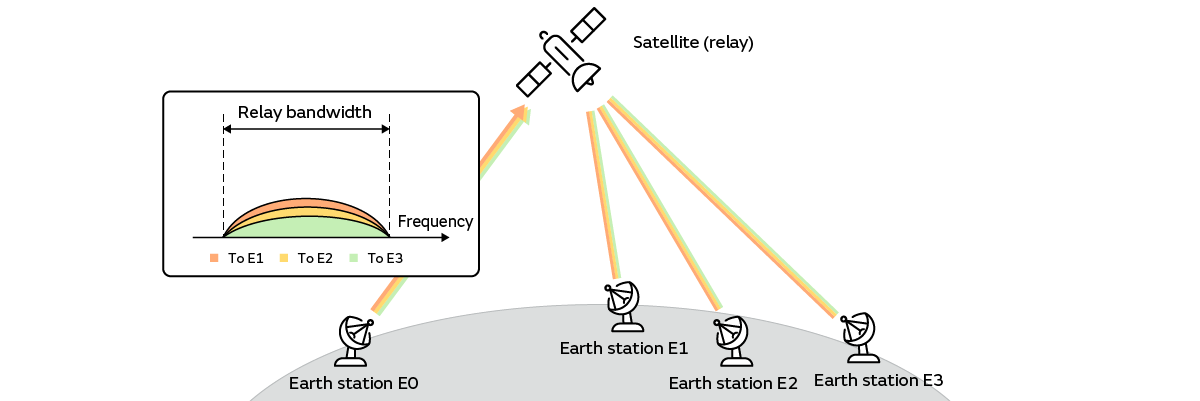
\includegraphics[width=0.85\textwidth]{images/fdma_example.png}
    \caption{FDMA resource allocation example.}
\end{figure}

\subsection{Time Division Multiple Access (TDMA)}
TDMA divides time into slots. Each user is given a dedicated time slot in a cyclic manner.

\begin{figure}[H]
    \centering
    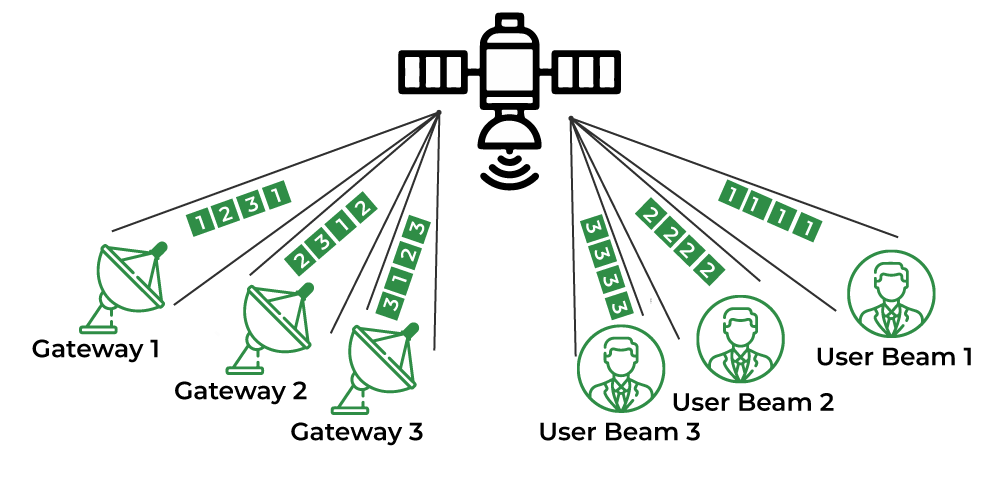
\includegraphics[width=0.85\textwidth]{images/tdma_example.png}
    \caption{TDMA time-slot allocation.}
\end{figure}

\subsection{Orthogonal Frequency Division Multiple Access (OFDMA)}
OFDMA is widely used in 4G and 5G systems. It divides the spectrum into many subcarriers and assigns them orthogonally to users.

\begin{equation}
X_k = \sum_{n=0}^{N-1} x_n e^{-j2\pi kn/N}
\end{equation}

Where:
\begin{itemize}
  \item $X_k$ is the $k$-th subcarrier symbol
  \item $x_n$ is the data on subcarrier $n$
  \item $N$ is the total number of subcarriers
\end{itemize}

\subsection{Non-Orthogonal Multiple Access (NOMA)}
NOMA allows multiple users to share the same time-frequency resources by using power-domain multiplexing and successive interference cancellation (SIC).

\begin{figure}[H]
    \centering
    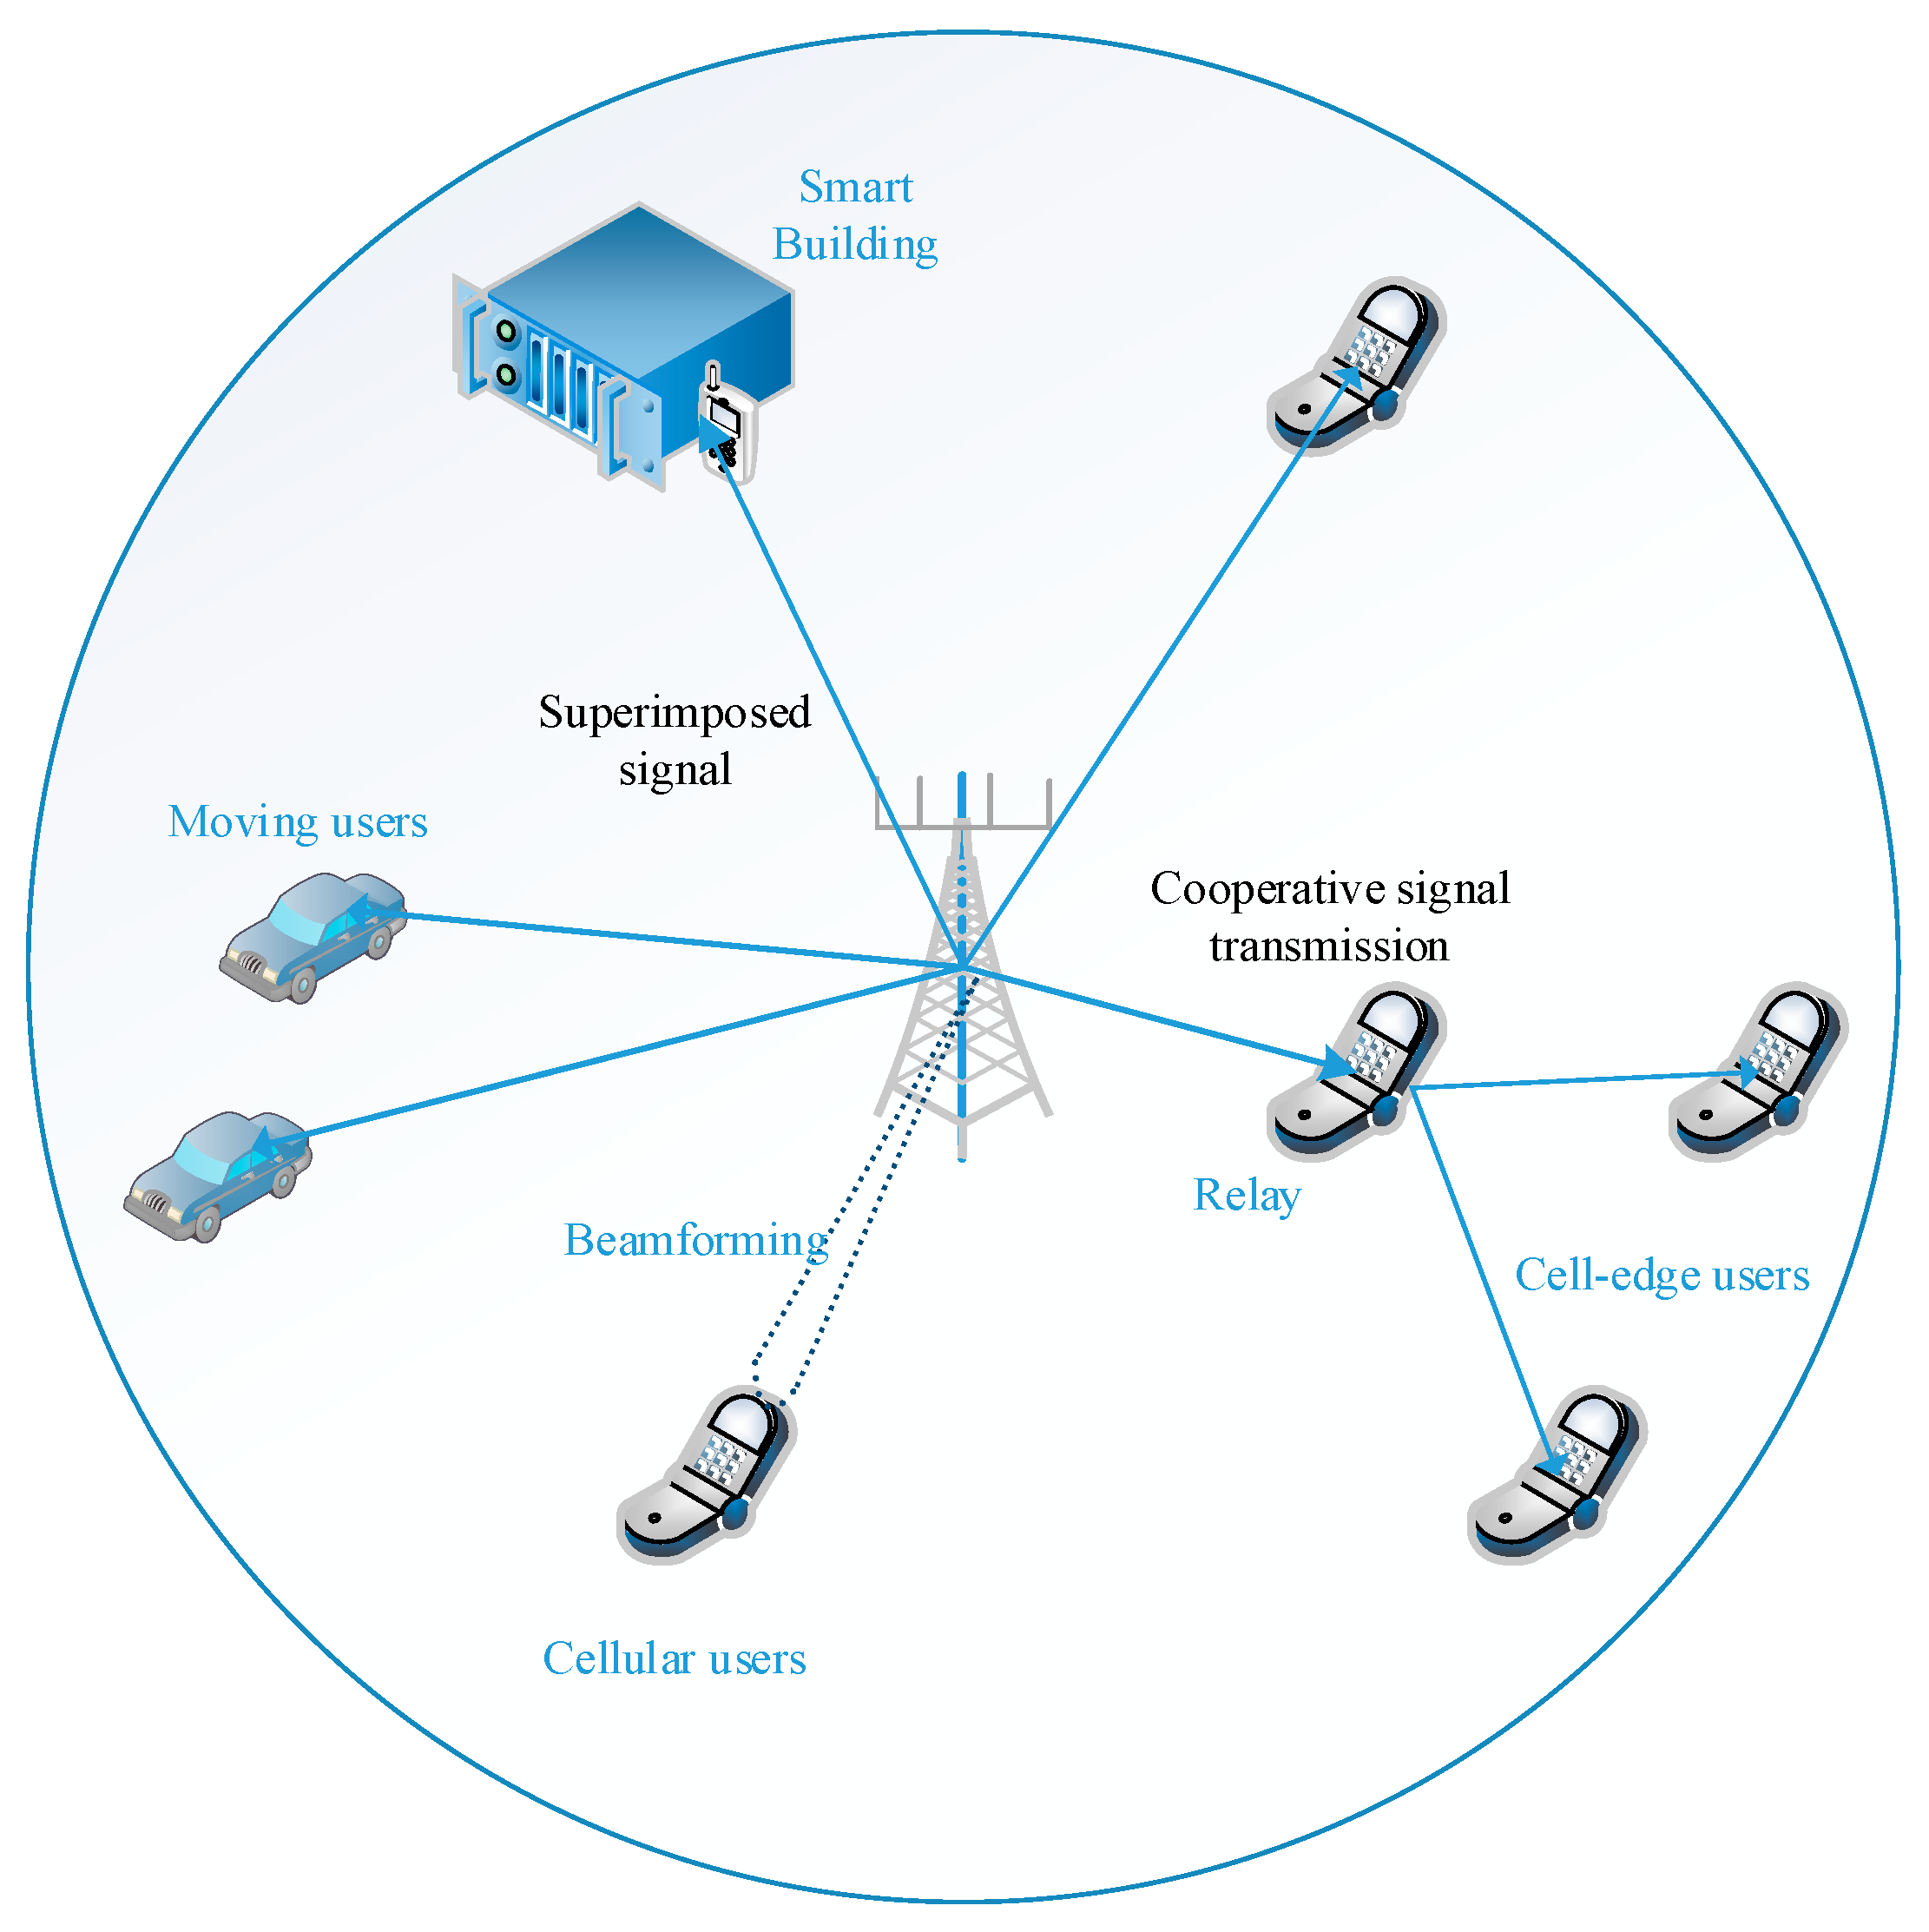
\includegraphics[width=0.75\textwidth]{images/noma_example.png}
    \caption{NOMA with successive interference cancellation.}
\end{figure}

\section{Scheduling Strategies}

\subsection{Round Robin (RR) Scheduler}
This scheduler allocates time slots to users in a cyclic order, ensuring fairness but not necessarily optimizing throughput.

\subsection{Proportional Fair (PF) Scheduler}
PF scheduler attempts to balance fairness and throughput. The metric is defined as:

\begin{equation}
M_i = \frac{R_i(t)}{\bar{R}_i(t)}
\end{equation}

Where:
\begin{itemize}
  \item $R_i(t)$ is the instantaneous rate of user $i$
  \item $\bar{R}_i(t)$ is the historical average rate
\end{itemize}

\section{Comparative Overview}

\begin{table}[H]
\centering
\begin{tabular}{|l|l|l|}
\hline
\textbf{Scheme} & \textbf{Orthogonal} & \textbf{Used In} \\
\hline
FDMA & Yes & 1G \\
TDMA & Yes & 2G \\
OFDMA & Yes & 4G, 5G \\
NOMA & No & 5G, 6G \\
\hline
\end{tabular}
\caption{Comparison of multiple access techniques.}
\end{table}

\section{Conclusion}
Multiple access and scheduling techniques form the backbone of cellular systems. Understanding their principles allows for better network optimization and user experience.

\vspace{1em}
\noindent\textbf{Next:} Appendix section includes hands-on simulations using Jupyter notebooks and Streamlit apps.

   % Week 3
% #📘 Chapter4_ChannelEstimationEqualization.tex

\chapter{Channel Estimation and Equalization}

\section{Introduction}
In a wireless communication system, signals propagate through a channel that introduces distortion due to multipath fading, noise, and Doppler shifts. To reliably decode the transmitted data, the receiver must estimate the channel and apply equalization techniques to mitigate these effects.

\section{Channel Effects}

\subsection{Multipath Fading}
A transmitted signal reaches the receiver through multiple paths, causing constructive and destructive interference.

\begin{itemize}
  \item Delay spread leads to Inter-Symbol Interference (ISI)
  \item Coherence bandwidth determines frequency selectivity
\end{itemize}

\subsection{Noise and Doppler Effects}
The wireless channel also adds additive white Gaussian noise (AWGN) and may cause Doppler shift due to user mobility.

\section{Channel Models}

\subsection{Flat Fading vs. Frequency Selective Fading}
\begin{itemize}
  \item Flat fading: Channel gain is constant across bandwidth
  \item Frequency selective fading: Channel varies across subcarriers
\end{itemize}

\subsection{Mathematical Model}
For a baseband channel:
\[
r(t) = h(t) * s(t) + n(t)
\]
Where:
\begin{itemize}
  \item $r(t)$ is the received signal
  \item $h(t)$ is the channel impulse response
  \item $s(t)$ is the transmitted signal
  \item $n(t)$ is additive noise
\end{itemize}

\section{Channel Estimation Techniques}

\subsection{Pilot-Based Estimation}
Transmit known pilot symbols at predefined locations. Estimate channel response based on received pilot values.

\[
\hat{h} = \frac{y_p}{x_p}
\]

\subsection{Least Squares (LS) Estimation}
Minimizes the squared error between received and estimated values.

\[
\hat{h}_{LS} = (X^H X)^{-1} X^H y
\]

\subsection{Minimum Mean Squared Error (MMSE) Estimation}
Takes noise and channel statistics into account.

\[
\hat{h}_{MMSE} = R_{hy} R_{yy}^{-1} y
\]

\section{Equalization Techniques}

\subsection{Zero Forcing Equalizer (ZF)}
Inverts the channel matrix assuming no noise.

\[
\hat{x} = (H^H H)^{-1} H^H y
\]

\subsection{MMSE Equalizer}
Balances inversion and noise suppression.

\[
\hat{x}_{MMSE} = (H^H H + \sigma^2 I)^{-1} H^H y
\]

\section{OFDM Channel Estimation}
OFDM uses pilot subcarriers across time and frequency.

\begin{figure}[H]
    \centering
    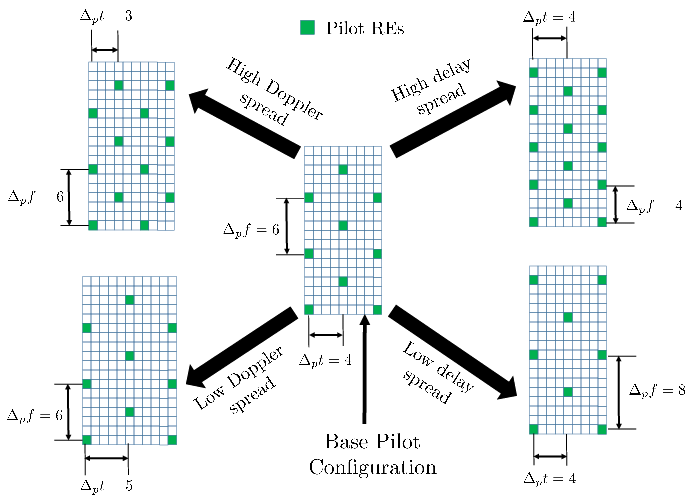
\includegraphics[width=0.7\textwidth]{images/ofdm_pilot_grid.png}
    \caption{Pilot placement in time-frequency grid of OFDM.}
\end{figure}

\section{Conclusion}
Accurate channel estimation and equalization are crucial for reliable communication in fading environments. In modern systems like 5G, advanced equalizers are paired with MIMO and OFDM to enhance performance.

\section*{Further Reading}
\begin{itemize}
  \item Rappaport, T. S. (2010). \textit{Wireless Communications: Principles and Practice}.
  \item Tse, D., \& Viswanath, P. (2005). \textit{Fundamentals of Wireless Communication}.
\end{itemize}

   % Week 4
% #📘 Chapter 5: MIMO \& Beamforming

\chapter{MIMO and Beamforming}

\section{Introduction to MIMO Systems}
Multiple-Input Multiple-Output (MIMO) is a fundamental technology in modern wireless communication systems, enabling high data rates and improved reliability. By using multiple antennas at both the transmitter and receiver, MIMO exploits multipath propagation to improve link capacity and robustness.

\section{Spatial Multiplexing}
Spatial multiplexing allows multiple data streams to be transmitted simultaneously over the same frequency band, effectively increasing the spectral efficiency. Each stream is transmitted from a different antenna and ideally received without interference.

\section{Diversity Gain vs. Multiplexing Gain}
\subsection{Diversity Gain}
Improves reliability by sending the same data across multiple antennas.

\subsection{Multiplexing Gain}
Increases capacity by transmitting independent data streams.

The diversity-multiplexing tradeoff must be carefully considered during system design.

\section{Channel Capacity of MIMO}
For an $N_t \times N_r$ MIMO system, the channel capacity is given by:
\[
C = \log_2 \det \left( I + \frac{\rho}{N_t} HH^H \right) \text{ bits/s/Hz}
\]
where $H$ is the channel matrix, $\rho$ is the SNR, and $H^H$ is the Hermitian transpose.

\section{Beamforming Concepts}
\subsection{Analog Beamforming}
Single RF chain, phase shifters applied in analog domain.

\subsection{Digital Beamforming}
Each antenna has its own RF chain, allowing full spatial control.

\subsection{Hybrid Beamforming}
Combines analog and digital techniques to reduce hardware complexity while maintaining performance.

\section{Antenna Arrays and Steering Vectors}
Beamforming is implemented by adjusting the phases across antenna elements. For a Uniform Linear Array (ULA), the steering vector for angle $\theta$ is:
\[
\mathbf{a}(\theta) = \left[1, e^{-jkd\sin(\theta)}, \ldots, e^{-jkd(N-1)\sin(\theta)} \right]^T
\]

\section{Practical Exploration (See Appendix)}
A detailed simulation and visualization of MIMO and beamforming concepts is provided in the accompanying Jupyter notebook and optional Streamlit app.

\section{References and Further Reading}
\begin{itemize}
  \item Goldsmith, A. (2005). \textit{Wireless Communications}. Cambridge University Press.
  \item Tse, D., \& Viswanath, P. (2005). \textit{Fundamentals of Wireless Communication}.
  \item Heath, R. W., \& Lozano, A. (2018). \textit{Foundations of MIMO Communication}.
  \item \texttt{https://web.mit.edu/6.450/www/} – Advanced Digital Communication resources.
\end{itemize}

\section{Appendix: Notebook and Streamlit App}
\begin{itemize}
  \item \textbf{Notebook:} \texttt{A5\_mimo\_beamforming\_simulation.ipynb} includes MIMO capacity simulations, beam pattern visualizations, and interactive antenna exploration.
  \item \textbf{Streamlit App:} \texttt{BeamPatternVisualizer.py} (optional) enables real-time exploration of beamforming patterns under different configurations.
\end{itemize}
   % Week 5
% 📘 Chapter 6: Massive MIMO & mmWave

\chapter{Massive MIMO \& mmWave Communication}

Massive MIMO and millimeter-wave (mmWave) technologies form the backbone of modern 5G and future 6G wireless systems. This chapter introduces the fundamentals of these technologies, explores the associated mathematical models, and demonstrates their benefits and limitations through examples.

\section{Introduction to Massive MIMO}

Massive MIMO refers to wireless communication systems with an extremely large number of antennas (typically tens to hundreds) at the base station. The primary goals are:

\begin{itemize}
  \item Increased spectral efficiency through spatial multiplexing.
  \item Improved energy efficiency by focusing transmission energy.
  \item Reduced interference via beamforming and spatial separation.
\end{itemize}

\subsection{Key Benefits}
\begin{itemize}
  \item \textbf{Channel hardening:} With more antennas, small-scale fading averages out.
  \item \textbf{Favorable propagation:} Orthogonality between channels of different users.
  \item \textbf{High capacity:} Significant data rate improvements under line-of-sight (LoS) and rich scattering.
\end{itemize}

\section{mmWave Communication Fundamentals}

Millimeter-wave (mmWave) bands typically refer to the frequency range between 24 GHz and 100 GHz. They are critical for high-bandwidth communication, enabling:

\begin{itemize}
  \item Multi-gigabit-per-second data rates.
  \item Dense spectrum reuse due to narrow beams.
  \item Compact antenna arrays because of small wavelengths.
\end{itemize}

\subsection{Challenges}
\begin{itemize}
  \item Severe free-space path loss (FSPL).
  \item High susceptibility to blockages and weather.
  \item Hardware complexity in RF chains and beamforming.
\end{itemize}

\section{Propagation at mmWave Frequencies}

Propagation characteristics at mmWave include:
\begin{itemize}
  \item High reflection and scattering.
  \item Poor diffraction around obstacles.
  \item Shorter range compared to sub-6GHz.
\end{itemize}

Despite these, mmWave communication benefits from the ability to use large antenna arrays to steer beams and concentrate energy.

\section{Beamforming: Analog, Digital, Hybrid}

\begin{itemize}
  \item \textbf{Analog beamforming:} Uses phase shifters at RF level.
  \item \textbf{Digital beamforming:} Baseband processing with each antenna connected to its own RF chain.
  \item \textbf{Hybrid beamforming:} Combination of both to reduce hardware complexity while retaining flexibility.
\end{itemize}

\section{MIMO Channel Capacity}

The capacity of a MIMO system increases with the number of antennas and SNR. For a MIMO system with \( N_t \) transmit and \( N_r \) receive antennas:

\[
C = \log_2 \det \left( I + \frac{P}{N_t N_0} H H^H \right)
\]

Where \( H \) is the channel matrix and \( P \) is the transmit power.

\section{Use Cases}

\begin{itemize}
  \item Fixed Wireless Access (FWA)
  \item Ultra-HD video streaming
  \item Wireless backhaul
  \item Vehicle-to-Everything (V2X)
\end{itemize}

\section{Summary}

\begin{itemize}
  \item Massive MIMO provides large gains in throughput and reliability by leveraging large antenna arrays.
  \item mmWave frequencies offer huge bandwidths but face path loss and blockage issues.
  \item Hybrid beamforming and smart antenna design are essential to realize these systems.
\end{itemize}

\section{Further Reading}
\begin{itemize}
  \item Marzetta, T. L., et al. ``Fundamentals of Massive MIMO.''
  \item Heath, R. W., et al. ``Millimeter Wave Wireless Communications.''
  \item 3GPP TR 38.900: Study on channel model for frequencies above 6 GHz.
\end{itemize}



   % Week 6
% \input{./chapters/topic7.tex}   % Week 7
% \input{./chapters/topic8.tex}   % Week 8: Exercises

% \input{./modules/week01_intro5G6G.tex}  % Week 1: Introduction
% \input{./modules/week02_5G_architecture.tex}   % Week 2
% \input{./modules/week03_radio_networks.tex}    % Week 3
% \input{./modules/week04_5G_applications.tex}   % Week 4
% \input{./modules/week05_beyond5G.tex}          % Week 5
% \input{./modules/week06_intro6G.tex}           % Week 6
% \input{./modules/week07_6G_AIblockchain.tex}   % Week 7
% \input{./modules/week08_exercises.tex}         % Week 8: Exercises
\clearpage

\appendix
% \appendix

\chapter{Appendix: Signal Strength and Path Loss Visualization}

\section{Overview}
This appendix introduces practical visualization of signal strength decay over distance using:
\begin{itemize}
  \item Free Space Path Loss (FSPL)
  \item Log-distance Path Loss model
\end{itemize}

\section{Simulation}
We provide both a Jupyter notebook and an interactive Streamlit app for hands-on exploration.

%\#✅ LaTeX Code to Embed FSPL Plot\#

\begin{figure}[H]
    \centering
    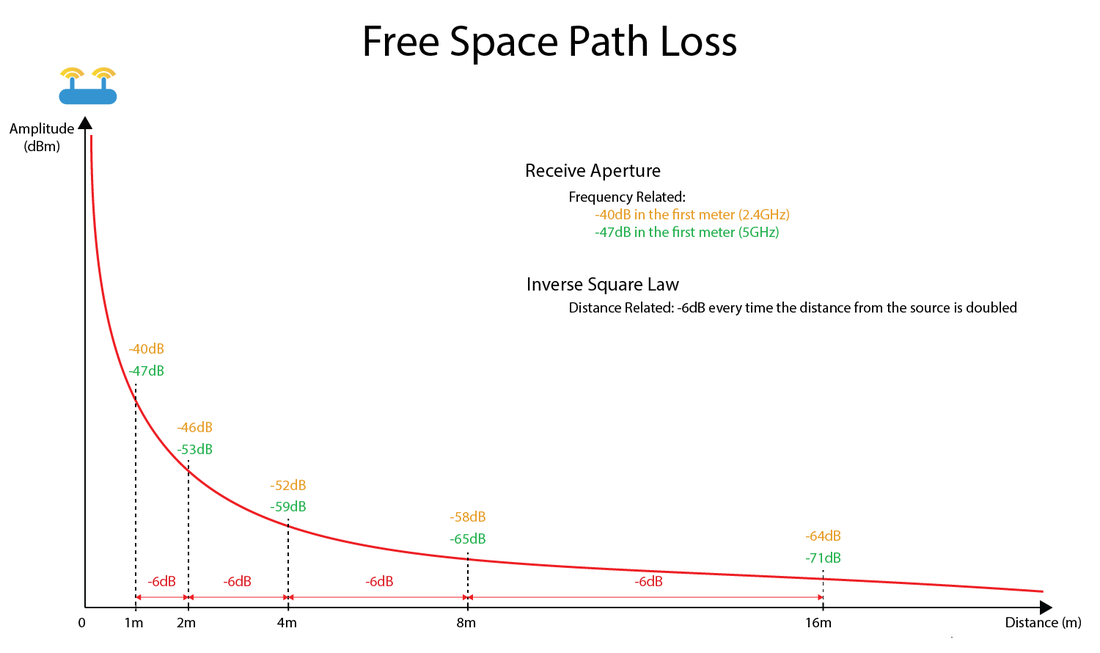
\includegraphics[width=0.85\textwidth]{./figures/fspl_plot.png}
    \caption{Free Space and Log-distance Path Loss vs. Distance}
    \label{fig:fspl_log_loss}
\end{figure}

\subsection{Notebook}
The notebook visualizes path loss vs. distance.

\textbf{Download:}
\begin{itemize}
  \item \href{run:./notebooks/A1-signal_strength.ipynb}{Jupyter Notebook (A1)}
  \item \href{run:./figures/fspl_plot.png}{Generated Path Loss Plot}
\end{itemize}

\subsection{Interactive Streamlit App}
The following app allows real-time manipulation of key parameters:
\begin{itemize}
  \item Frequency (GHz)
  \item Maximum Distance
  \item Path Loss Exponent
\end{itemize}

\textbf{Link:} \href{http://<your-deployed-url>:8501}{Open Signal Visualizer App}

\section{References}
\begin{enumerate}
  \item Rappaport, T. S. (2014). \textit{Wireless Communications: Principles and Practice}.
  \item 3GPP Technical Specification TS 36.942.
  \item Fundamentals of 5G Mobile Networks – Wiley.
\end{enumerate}

% \appendix

\chapter{Appendix: Modulation and Spectrum Simulation}

\section{Interactive OFDM Simulation Notebook}

To solidify the understanding of OFDM signal structure and spectral characteristics, an interactive Python notebook titled \texttt{A2-ofdm\_simulation.ipynb} is provided. This notebook allows learners to:

\begin{itemize}
  \item Visualize subcarriers of OFDM symbols.
  \item Explore Inverse Fast Fourier Transform (IFFT) as a modulation mechanism.
  \item Understand the effect of symbol length and guard intervals.
  \item Plot time and frequency domain representations.
\end{itemize}

\textbf{Notebook Access:}  
You can download the notebook from the following location:  
\url{<YOUR-LINK-TO-NOTEBOOK>}

\subsection{Modulation Scheme Explorer (Optional Streamlit App)}

For learners who prefer hands-on exploration, an interactive web application \texttt{ModulationExplorer.py} is also available. It allows users to experiment with:

\begin{itemize}
  \item QPSK, 16-QAM, and 64-QAM constellations.
  \item Variable number of symbols and noise levels.
  \item Visualization of signal degradation due to noise.
\end{itemize}

\begin{figure}[h!]
  \centering
  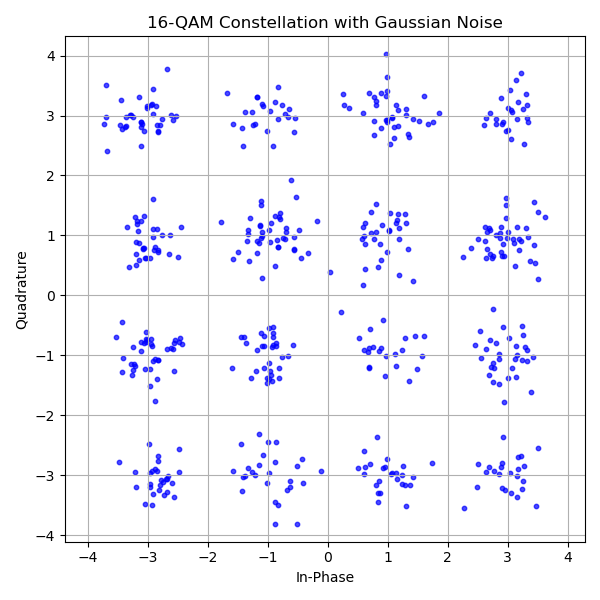
\includegraphics[width=0.8\textwidth]{figures/modulation_constellation_example.png}
  \caption{Example QAM constellation with added Gaussian noise (from Streamlit app).}
  \label{fig:modulation-app}
\end{figure}

\textbf{App Access:}  
Run the Streamlit app using the following command:
\begin{verbatim}
streamlit run ModulationExplorer.py
\end{verbatim}

\textbf{App Download:}  
\url{<YOUR-LINK-TO-APP-CODE>}

\subsection{Learning Outcomes}

\begin{itemize}
  \item Experience the spectral efficiency of OFDM in practice.
  \item Understand modulation scheme differences in terms of constellation design and noise resilience.
  \item Gain intuition about bit-symbol mappings and symbol space in the IQ-plane.
\end{itemize}

\textbf{Recommended Exercises:}
\begin{enumerate}
  \item Modify the number of subcarriers in the OFDM notebook and observe spectral changes.
  \item Change modulation order in the Streamlit app and analyze BER qualitatively.
\end{enumerate}

% \appendix

\chapter{Appendix: Multiple Access and Scheduling Simulations}

\subsection{A3\_multiple\_access\_simulation.ipynb}

This Jupyter notebook demonstrates various multiple access techniques such as FDMA, TDMA, OFDMA, and NOMA using interactive Python visualizations. It includes practical implementations of:

\begin{itemize}
  \item Frequency division and time division allocation
  \item Subcarrier mapping in OFDMA
  \item Power-domain multiplexing in NOMA
  \item Basic scheduler logic for Round Robin and Proportional Fair algorithms
\end{itemize}

\noindent You can run and interact with the notebook directly via:

\begin{itemize}
  \item \textbf{Notebook GitHub link:} \url{https://github.com/your-repo/5G6G-course/blob/main/notebooks/A3_multiple_access_simulation.ipynb}
  \item \textbf{View online (via nbviewer):} \url{https://nbviewer.org/github/your-repo/5G6G-course/blob/main/notebooks/A3_multiple_access_simulation.ipynb}
\end{itemize}

\vspace{1em}
\subsection{SchedulerVisualizer.py (Streamlit App)}

To allow real-time interaction and exploration, we have also developed a dedicated Streamlit web app for this chapter.

This app provides:
\begin{itemize}
  \item Interactive sliders to simulate TDMA/FDMA/OFDMA with customizable users and resources
  \item A visual explanation of NOMA’s power domain allocation
  \item Simulated round-robin and proportional fair scheduler behavior
\end{itemize}

\noindent Run the app locally with:

\begin{verbatim}
streamlit run SchedulerVisualizer.py
\end{verbatim}

Or visit the hosted version here:

\begin{itemize}
  \item \textbf{Live app:} \url{https://your-app-hosting-url.com/SchedulerVisualizer}
\end{itemize}

\vspace{1em}
\subsection{Figures Used in This Chapter}

\vspace{1em}
\begin{figure}[H]
  \centering
  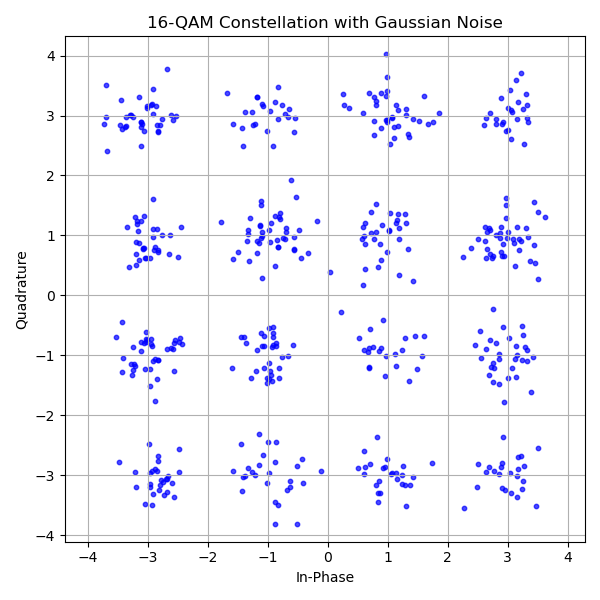
\includegraphics[width=0.85\textwidth]{./figures/modulation_constellation_example.png}
  \caption{Example modulation constellation diagram, used in Chapter 2 and referenced in scheduler visualizations.}
\end{figure}

\newpage

% \appendix

% #📘 appendix-ch4-channel-estimation-equalization.tex

\chapterAppendix: Channel Estimation and Equalization}
%\label{appendix:channel_estimation}

This appendix supplements Chapter 4 by providing a practical demonstration of channel estimation and equalization techniques used in modern OFDM systems like LTE and 5G NR.

\subsection{Notebook Simulation: \texttt{A4\_channel\_equalization.ipynb}}

The notebook implements the following:

\begin{itemize}
  \item QPSK modulation over 64 OFDM subcarriers.
  \item Addition of a cyclic prefix and multipath channel convolution.
  \item Complex AWGN noise addition.
  \item Channel estimation using Least Squares (LS) method.
  \item Equalization and recovery of original QPSK symbols.
\end{itemize}

The simulation assumes pilot-based LS estimation and perfect channel knowledge at the receiver for educational clarity.

\subsection{Streamlit App (Optional)}
For interactive learning, a Streamlit-based simulation page may be included in the modular app to vary parameters like channel taps, SNR, and modulation order.

\subsection{Visualization of Equalized Symbols}

Figure~\ref{fig:equalized-constellation} shows the scatter plot of the received frequency-domain symbols and the equalized output after applying channel estimation.

\begin{figure}[H]
    \centering
    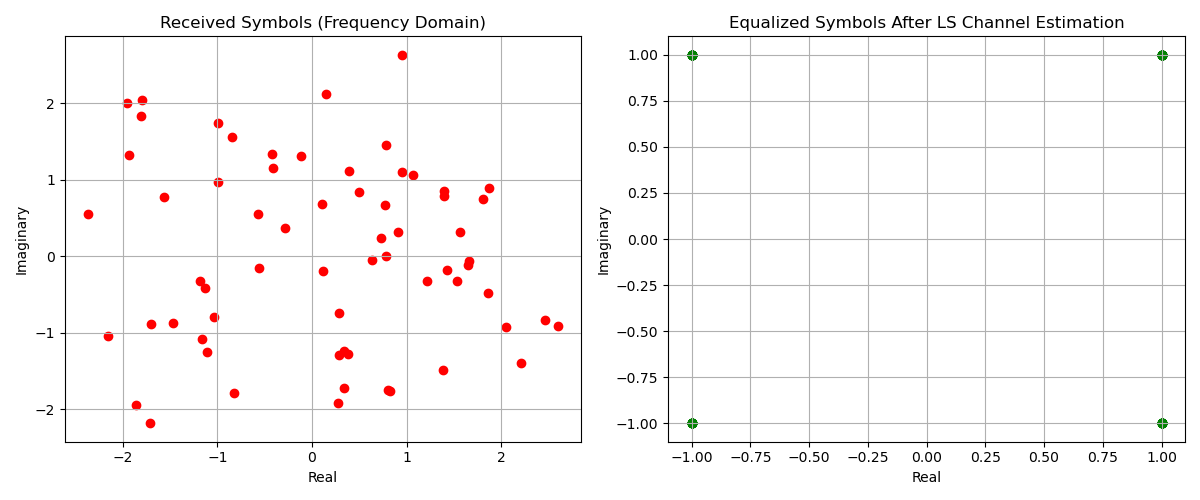
\includegraphics[width=0.75\textwidth]{./figures/equalized_constellation.png}
    \caption{Constellation plot of received vs. equalized QPSK symbols.}
    \label{fig:equalized-constellation}
\end{figure}

\subsection*{References}
\begin{enumerate}
    \item Rappaport, T. S. \textit{Wireless Communications: Principles and Practice}, Pearson.
    \item Goldsmith, A. \textit{Wireless Communications}, Cambridge University Press.
    \item Proakis, J. G., \textit{Digital Communications}.
    \item 3GPP TS 36.211: \textit{Physical Channels and Modulation (LTE)}.
\end{enumerate}



\section{Additional Appendix: Channel Estimation and Equalization Simulation}

\subsection{Overview}

This appendix provides a hands-on simulation of OFDM-based channel estimation and equalization using a simple multipath fading channel. The exercises are aimed at helping learners visualize the distortion introduced by the wireless channel and how equalization can recover the original signal.

\subsection{Interactive Notebook: \texttt{A4\_channel\_equalization.ipynb}}

The Jupyter Notebook implements the following:
\begin{itemize}
  \item Generation of QPSK-modulated OFDM symbols
  \item Simulation of a multipath channel with user-defined tap coefficients
  \item Addition of AWGN noise based on a tunable SNR
  \item Least Squares (LS) channel estimation
  \item Equalization of the received signal
  \item Scatter plots comparing received and equalized symbols
\end{itemize}

\noindent
You can access and run the notebook here:

\begin{quote}
\texttt{[Download or open from: A4\_channel\_equalization.ipynb]}
\end{quote}

\subsection{Streamlit App: EqualizerSimulator.py}

A lightweight web interface allows learners to interactively tune parameters like:
\begin{itemize}
  \item Number of subcarriers ($N$)
  \item Cyclic prefix length
  \item SNR (dB)
  \item Complex channel tap coefficients
\end{itemize}

\noindent
Launch the app locally or via cloud deployment to visualize the following:
\begin{enumerate}
  \item Received symbols (with distortion)
  \item Equalized symbols (recovered)
\end{enumerate}

\noindent
\textbf{To launch locally:}
\begin{verbatim}
 streamlit run EqualizerSimulator.py
\end{verbatim}

\subsection{Example Constellation Plot}

\begin{figure}[H]
  \centering
  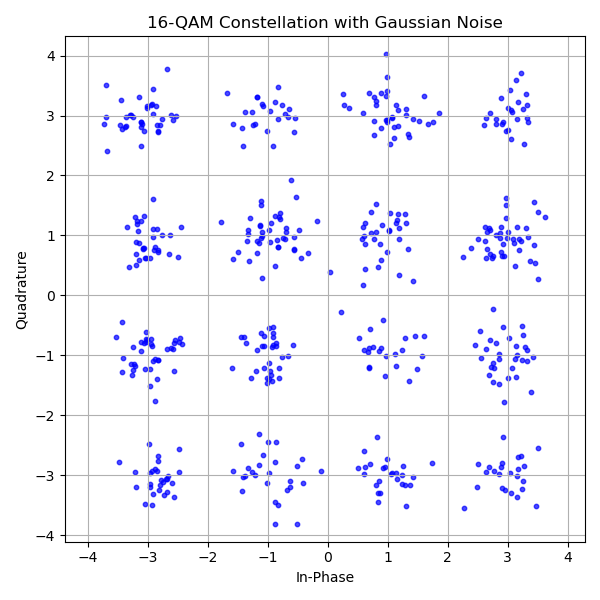
\includegraphics[width=0.7\textwidth]{./figures/modulation_constellation_example.png}
  \caption{Comparison of Received vs Equalized QPSK Symbols}
  \label{fig:equalized_qpsk}
\end{figure}

\subsection{References}
\begin{itemize}
  \item S. Haykin and M. Moher, \textit{Modern Wireless Communications}, Pearson
  \item T. S. Rappaport, \textit{Wireless Communications: Principles and Practice}, Prentice Hall
  \item 3GPP Technical Reports on OFDM and Channel Estimation
  \item MATLAB and Python tutorials on Least Squares Estimation
\end{itemize}


% # ✅ Features:
%  * Adjustable SNR, Cyclic Prefix, and Channel Taps.
%  * Visual comparison: Received symbols vs Equalized symbols.
%  * Uses Least Squares Estimation for channel response.

% \appendix

% 📘 appendix-A5-mimo-and-beamforming-simulation.tex

\chapter{Appendix: MIMO \& Beamforming Simulation}

\section{MIMO \& Beamforming Simulation}

\subsection{Overview}
This appendix supplements Chapter 5 by providing simulation code and interactive visualizations to reinforce understanding of key MIMO and beamforming concepts.

\subsection{Jupyter Notebook: MIMO and Beamforming Simulation}

The notebook \texttt{A5\_mimo\_beamforming\_simulation.ipynb} covers the following topics:

\begin{itemize}
    \item Simulation of a MIMO channel
    \item Calculation of MIMO channel capacity
    \item Beamforming weight computation
    \item Visualization of antenna beam patterns
    \item Exploration of capacity scaling with antenna count
\end{itemize}

\noindent\textbf{Download notebook:} \\
\url{https://your-download-link.com/A5_mimo_beamforming_simulation.ipynb} \hfill (replace with actual link)

\begin{figure}[h!]
    \centering
    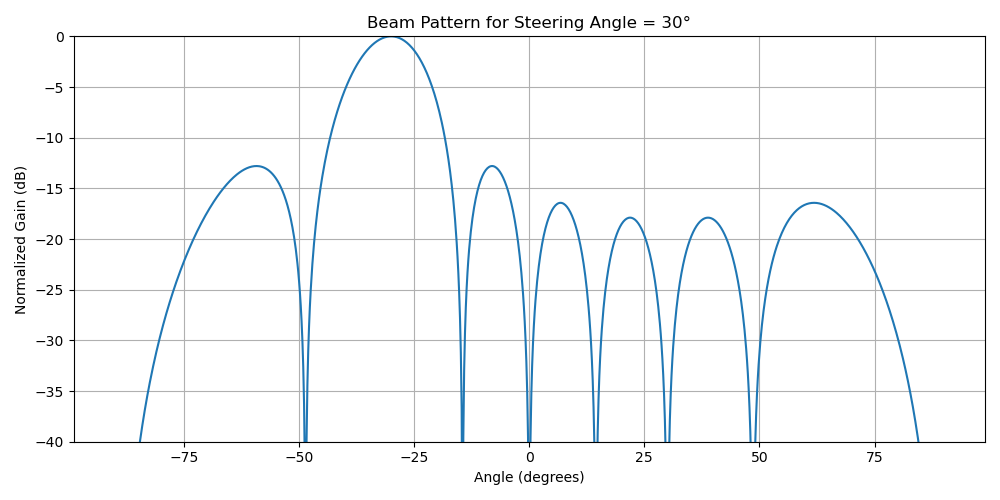
\includegraphics[width=0.9\textwidth]{./figures/beam_pattern_example.png}
    \caption{Example beam pattern for an 8-element uniform linear array steering at $30^\circ$}
    \label{fig:beam-pattern}
\end{figure}

\subsection{Interactive Streamlit App: Beam Pattern Visualizer}

An interactive app named \texttt{BeamPatternVisualizer.py} allows students to explore beamforming characteristics in real time.

\begin{itemize}
    \item Select number of antennas and spacing
    \item Adjust steering direction
    \item Switch between analog, digital, and hybrid beamforming
\end{itemize}

\noindent\textbf{Run app:} \\
\url{https://your-streamlit-link.com/BeamPatternVisualizer} \hfill (replace with actual deployed URL)

\subsection{Key Learnings}

\begin{itemize}
    \item Increasing the number of antennas enhances directionality and capacity
    \item Beamforming focuses signal energy toward desired directions
    \item Analog beamforming uses phase shifts only, while digital uses complex weights
    \item Hybrid beamforming provides a practical trade-off
\end{itemize}

\subsection{References}

\begin{itemize}
    \item T. L. Marzetta, ``Noncooperative Cellular Wireless with Unlimited Numbers of Base Station Antennas,'' IEEE Trans. Wireless Commun., 2010.
    \item A. Goldsmith, ``Wireless Communications,'' Cambridge University Press, 2005.
    \item D. Tse and P. Viswanath, ``Fundamentals of Wireless Communication,'' Cambridge University Press.
\end{itemize}

% \input{a./chapters/ppendix-A6.tex}

\clearpage



\thispagestyle{empty}



\vfill

% \begin{center}
% % \begin{textblock*}{297mm}(0mm,0mm)
%      
\includegraphics[width=0.85\textwidth, angle=0]{./figures/5g6g.png}
% % \end{textblock*}
% \end{center}

%%% The last page of the report
\clearpage
\pagecolor{stardustbg}
\thispagestyle{empty}
\begin{tikzpicture}[remember picture, overlay]
  \node[anchor=south west, inner sep=0] at (current page.south west) {
    
\includegraphics[width=\paperwidth]{./figures/5g6g.png} %,height=\paperheight
  }; 
\end{tikzpicture}
\clearpage

\clearpage
\end{document}